
\documentclass[a4paper,11pt]{article}
\usepackage[a4paper, margin=8em]{geometry}

% usa i pacchetti per la scrittura in italiano
\usepackage[french,italian]{babel}
\usepackage[T1]{fontenc}
\usepackage[utf8]{inputenc}
\frenchspacing 

% usa i pacchetti per la formattazione matematica
\usepackage{amsmath, amssymb, amsthm, amsfonts}

% usa altri pacchetti
\usepackage{gensymb}
\usepackage{hyperref}
\usepackage{standalone}

% imposta il titolo
\title{Appunti Fondamenti di Automatica}
\author{Luca Seggiani}
\date{2025}

% disegni
\usepackage{pgfplots}
\pgfplotsset{width=10cm,compat=1.9}

% imposta lo stile
% usa helvetica
\usepackage[scaled]{helvet}
% usa palatino
\usepackage{palatino}
% usa un font monospazio guardabile
\usepackage{lmodern}

% tikz in sans
\tikzset{every picture/.style={/utils/exec={\sffamily}}}

\renewcommand{\rmdefault}{ppl}
\renewcommand{\sfdefault}{phv}
\renewcommand{\ttdefault}{lmtt}

% circuiti
\usepackage{circuitikz}
\usetikzlibrary{babel}

% disponi il titolo
\makeatletter
\renewcommand{\maketitle} {
	\begin{center} 
		\begin{minipage}[t]{.8\textwidth}
			\textsf{\huge\bfseries \@title} 
		\end{minipage}%
		\begin{minipage}[t]{.2\textwidth}
			\raggedleft \vspace{-1.65em}
			\textsf{\small \@author} \vfill
			\textsf{\small \@date}
		\end{minipage}
		\par
	\end{center}

	\thispagestyle{empty}
	\pagestyle{fancy}
}
\makeatother

% disponi teoremi
\usepackage{tcolorbox}
\newtcolorbox[auto counter, number within=section]{theorem}[2][]{%
	colback=blue!10, 
	colframe=blue!40!black, 
	sharp corners=northwest,
	fonttitle=\sffamily\bfseries, 
	title=Teorema~\thetcbcounter: #2, 
	#1
}

% disponi definizioni
\newtcolorbox[auto counter, number within=section]{definition}[2][]{%
	colback=red!10,
	colframe=red!40!black,
	sharp corners=northwest,
	fonttitle=\sffamily\bfseries,
	title=Definizione~\thetcbcounter: #2,
	#1
}

% disponi problemi
\newtcolorbox[auto counter, number within=section]{problem}[2][]{%
	colback=green!10,
	colframe=green!40!black,
	sharp corners=northwest,
	fonttitle=\sffamily\bfseries,
	title=Problema~\thetcbcounter: #2,
	#1
}

% disponi codice
\usepackage{listings}
\usepackage[table]{xcolor}

\lstdefinestyle{codestyle}{
		backgroundcolor=\color{black!5}, 
		commentstyle=\color{codegreen},
		keywordstyle=\bfseries\color{magenta},
		numberstyle=\sffamily\tiny\color{black!60},
		stringstyle=\color{green!50!black},
		basicstyle=\ttfamily\footnotesize,
		breakatwhitespace=false,         
		breaklines=true,                 
		captionpos=b,                    
		keepspaces=true,                 
		numbers=left,                    
		numbersep=5pt,                  
		showspaces=false,                
		showstringspaces=false,
		showtabs=false,                  
		tabsize=2
}

\lstdefinestyle{shellstyle}{
		backgroundcolor=\color{black!5}, 
		basicstyle=\ttfamily\footnotesize\color{black}, 
		commentstyle=\color{black}, 
		keywordstyle=\color{black},
		numberstyle=\color{black!5},
		stringstyle=\color{black}, 
		showspaces=false,
		showstringspaces=false, 
		showtabs=false, 
		tabsize=2, 
		numbers=none, 
		breaklines=true
}

\lstdefinelanguage{javascript}{
	keywords={typeof, new, true, false, catch, function, return, null, catch, switch, var, if, in, while, do, else, case, break},
	keywordstyle=\color{blue}\bfseries,
	ndkeywords={class, export, boolean, throw, implements, import, this},
	ndkeywordstyle=\color{darkgray}\bfseries,
	identifierstyle=\color{black},
	sensitive=false,
	comment=[l]{//},
	morecomment=[s]{/*}{*/},
	commentstyle=\color{purple}\ttfamily,
	stringstyle=\color{red}\ttfamily,
	morestring=[b]',
	morestring=[b]"
}

% disponi sezioni
\usepackage{titlesec}

\titleformat{\section}
	{\sffamily\Large\bfseries} 
	{\thesection}{1em}{} 
\titleformat{\subsection}
	{\sffamily\large\bfseries}   
	{\thesubsection}{1em}{} 
\titleformat{\subsubsection}
	{\sffamily\normalsize\bfseries} 
	{\thesubsubsection}{1em}{}

% disponi alberi
\usepackage{forest}

\forestset{
	rectstyle/.style={
		for tree={rectangle,draw,font=\large\sffamily}
	},
	roundstyle/.style={
		for tree={circle,draw,font=\large}
	}
}

% disponi algoritmi
\usepackage{algorithm}
\usepackage{algorithmic}
\makeatletter
\renewcommand{\ALG@name}{Algoritmo}
\makeatother

% disponi numeri di pagina
\usepackage{fancyhdr}
\fancyhf{} 
\fancyfoot[L]{\sffamily{\thepage}}

\makeatletter
\fancyhead[L]{\raisebox{1ex}[0pt][0pt]{\sffamily{\@title \ \@date}}} 
\fancyhead[R]{\raisebox{1ex}[0pt][0pt]{\sffamily{\@author}}}
\makeatother

\begin{document}

% sezione (data)
\section{Lezione del 29-04-25}

% stili pagina
\thispagestyle{empty}
\pagestyle{fancy}

% testo
Riprendiamo il discorso sui diagrammi di Nyquist.

\subsubsection{Esempio: diagramma di Nqyuist}
Facciamo l'esempio del tracciamento del diagramma di Nyquist per la funzione di trasferimento:
$$
G(s) = \frac{1}{s^2 + 3s + 2}
$$
Il primo passo sarà chiaramente quello di trovare la funzione di risposta armonica:
$$
G(j \omega) = \frac{1}{-\omega^2 + 3 j \omega + 2}
$$
Vediamo quindi le risposte rispettivamente a $\omega \rightarrow 0$ e $\omega \rightarrow + \infty$:
\begin{itemize}
	\item $\omega \rightarrow 0$:
		$$
		\lim_{\omega \rightarrow 0} \frac{1}{-\omega^2 + 3 j \omega + 2} = \frac{1}{2} \, \angle \, 0^\circ
		$$
	\item $\omega \rightarrow +\infty$:
		$$
		\lim_{\omega \rightarrow +\infty} \frac{1}{-\omega^2 + 3 j \omega + 2} \Big|_{\omega \rightarrow + \infty} = 0^- \text{ cioè } 0 \, \angle \, -180^\circ
		$$
		o alternativamente applicando la regola vista in 22.1.1, punto 2:
		$$
		\phi_{\omega \rightarrow + \infty} = - 2 \cdot \frac{\pi}{2} = - \pi = -180^\circ
		$$
\end{itemize}

Vediamo quindi le intersezioni con gli assi.
Per valutarle razionalizziamo la $G(j \omega)$ in componente reale e immaginaria:
$$
G(j \omega) = x + j y = \frac{1}{(2 - \omega^2) + 3 j \omega} \cdot \frac{(2 - \omega^2) - 3 j \omega}{(2 - \omega^2) - 3 j \omega}
= \frac{(2 - \omega^2) - 3 j \omega}{(2 - \omega)^2 + 9 \omega^2}
$$

Poniamo quindi separatamente parte reale e immaginaria a 0:
\begin{itemize}
	\item $\mathrm{Re}(G(s)) = 0$:
		$$
			2 - \omega^2 = 0 \implies \omega = \sqrt{2}
		$$
		in quanto ci interessa solo la parte $\omega \in [0, +\infty)$.
		Sostituendo nella parte complessa si ha quindi:
		$$
		G(j\omega) = \frac{-3 j \sqrt{2}}{18} = -\frac{\sqrt{2}}{6} j 
		$$
	\item $\mathrm{Im}(G(s)) = 0$:
		$$
			-3 j \omega = 0 \implies \omega = 0
		$$
		Vediamo che abbiamo già considerato questo caso.
		Resta quindi solo la possibilità che il denominatore vada a infinito, cosa che si verifica per $\omega \rightarrow + \infty$, ma che ancora una volta abbiamo già considerato.
\end{itemize}

\noindent
\begin{minipage}{\textwidth}

Possiamo quindi procedere a tracciare il grafico mettendo in evidenza i punti trovati:
\begin{center}
	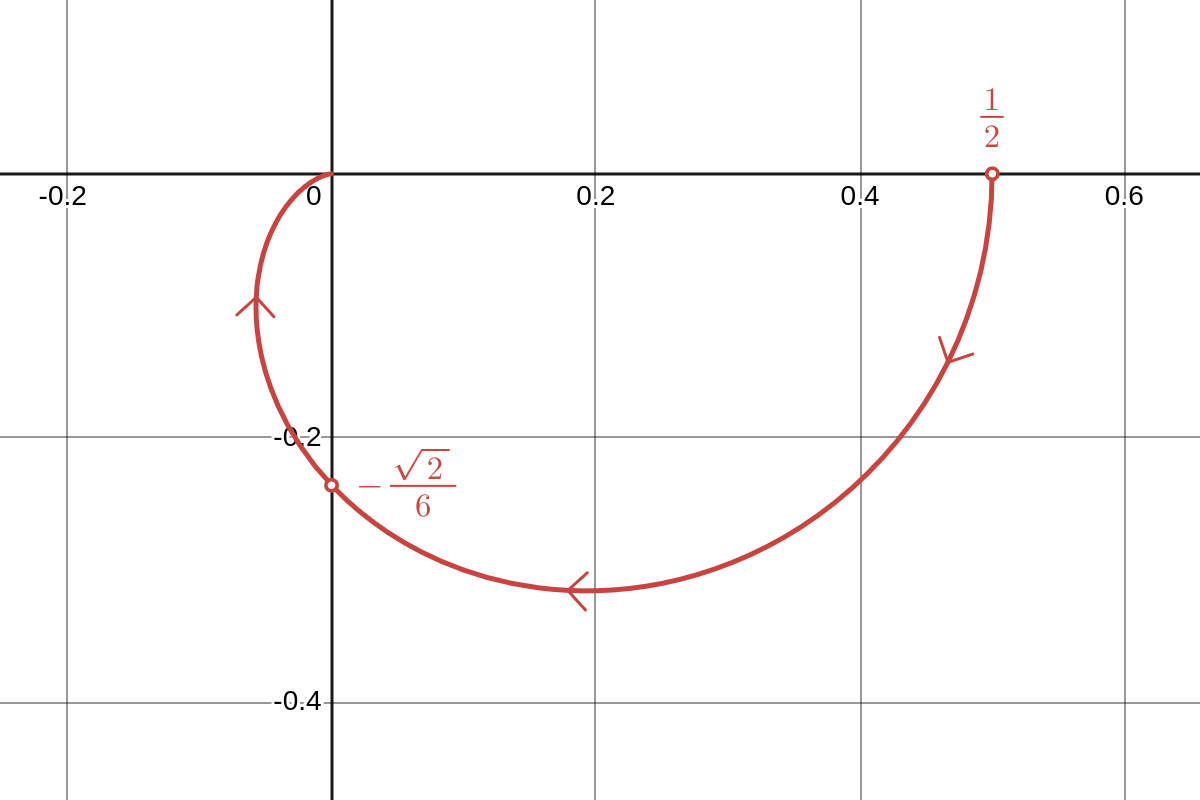
\includegraphics[scale=0.28]{../figures/nyquist/first_ex.png}
\end{center}

\end{minipage}

\subsubsection{Diagrammi di Nyquist da diagrammi di Bode}
Possiamo tracciare i diagrammi di Nyquist, in maniera qualitativa, a partire dalla conoscenza dei corrispondenti diagrammi di Bode, in modulo e fase.

Prendiamo a scopo di esempio la funzione di trasferimento:
$$
G(s) = \frac{K}{ (1 + s T_1) (1 + s T_2) (1 + s T_3) }
$$
da cui la funzione di risposta armonica:
$$
G(j \omega) = \frac{K}{ (1 + j \omega T_1) (1 + j \omega T_2) (1 + j \omega T_3) }
$$
Per quanto riguarda i limiti avremo:
\begin{itemize}
	\item $\omega \rightarrow 0$:
	$$
	G(0) = K \, \angle \, 0^\circ
	$$
	\item $\omega \rightarrow +\infty$:
	$$
	G(+ \infty) = 0^\circ, \quad \phi_{\omega \rightarrow + \infty} \sim \angle \frac{K}{(j \omega)^3} = -90^\circ \cdot 3 = -270^\circ
	$$
\end{itemize}

A questo punto possiamo tracciare informazioni aggiuntive tracciando i diagrammi di Bode di modulo e fase.
Abbiamo dalla funzione di risposta armonica che i termini:
$$
(1 + j \omega T_1), \quad (1 + j \omega T_2), \quad (1 + j \omega T_3)
$$
rappresentano 3 filtri passa basso con frequenze di taglio rispettivamente di $\frac{1}{T_1}$, $\frac{1}{T_2}$ e $\frac{1}{T_3}$.

\noindent
\begin{minipage}{\textwidth}

Il valore $K$ rappresenta invece una costante di $|K|_dB$, per cui il grafico complessivo del modulo è:
\begin{center}
	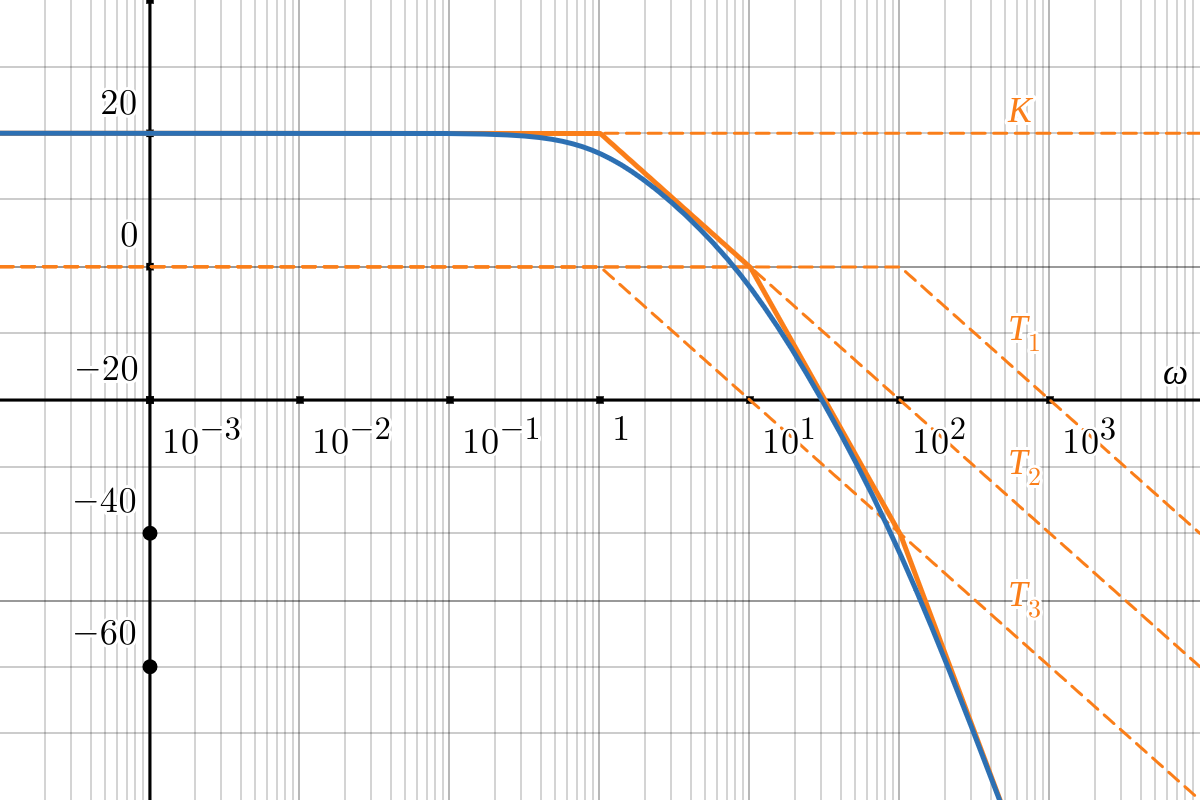
\includegraphics[scale=0.3]{../figures/nyquist/second_ex_1.png}
\end{center}

\end{minipage}

Per quanto riguarda la fase, abbiamo che i 3 filtri passa basso hanno scostamento presi singolarmente di $-90^\circ$, per cui lo scostamento in fase complessivo per $\omega >> 0$ è:
$$
-90^\circ \cdot 3 = -270^\circ
$$
e il grafico della fase risulta:
\begin{center}
	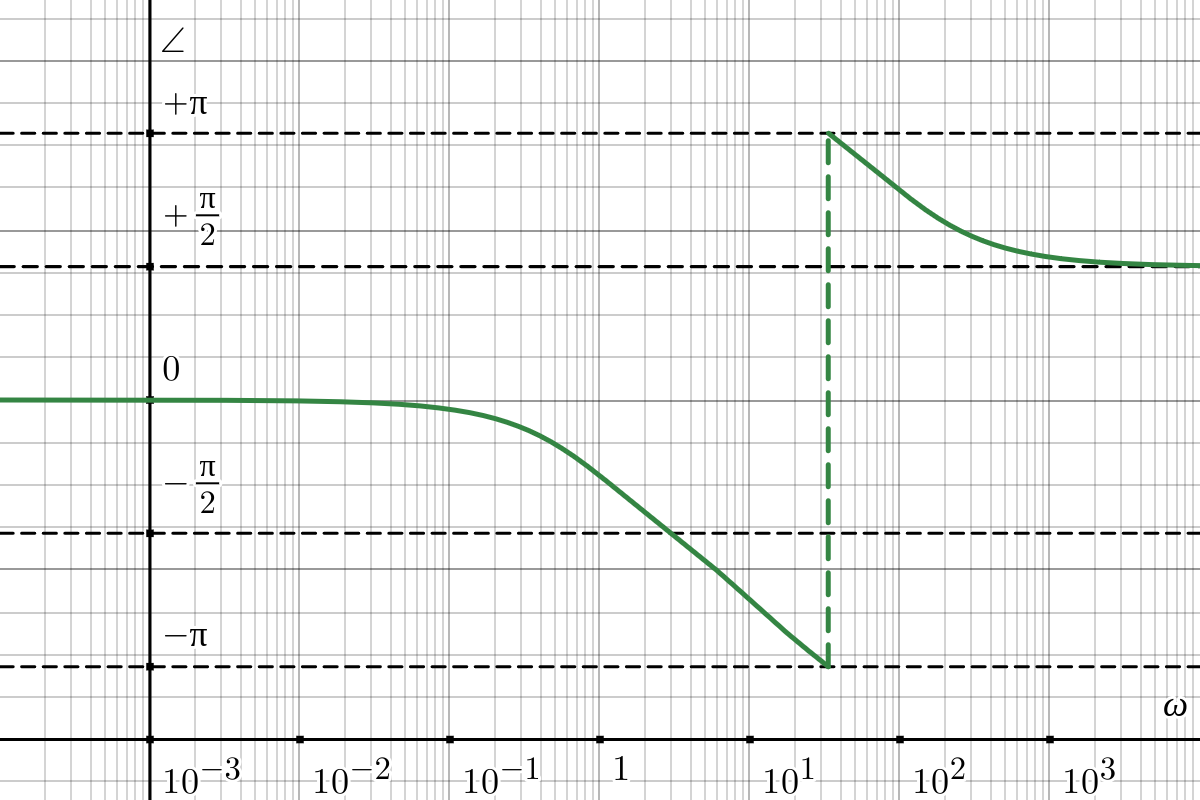
\includegraphics[scale=0.3]{../figures/nyquist/second_ex_2.png}
\end{center}

Vediamo quindi che abbiamo ricavato informazioni consistenti con quelle ottenute di limiti, in quanto:
\begin{itemize}
	\item Per quanto riguarda il modulo, i $|K|_{dB}$ del modulo a $\omega << 1$ equivalgono al modulo $|K|$ del limite in 0, mentre il limite a $+\infty$ va a $-\infty$ dB, cioè 0;
	\item Per quanto riguarda la fase, abbiamo ritrovato esattamente l'andamento da $0^\circ$ a $270^\circ$ descritto dai limiti.
\end{itemize}

Possiamo quindi sfruttare le informazioni sull'andamento intermedio di modulo e fase per tracciare il diagramma di Nyquist, che avrà un'aspetto del tipo:
\begin{center}
	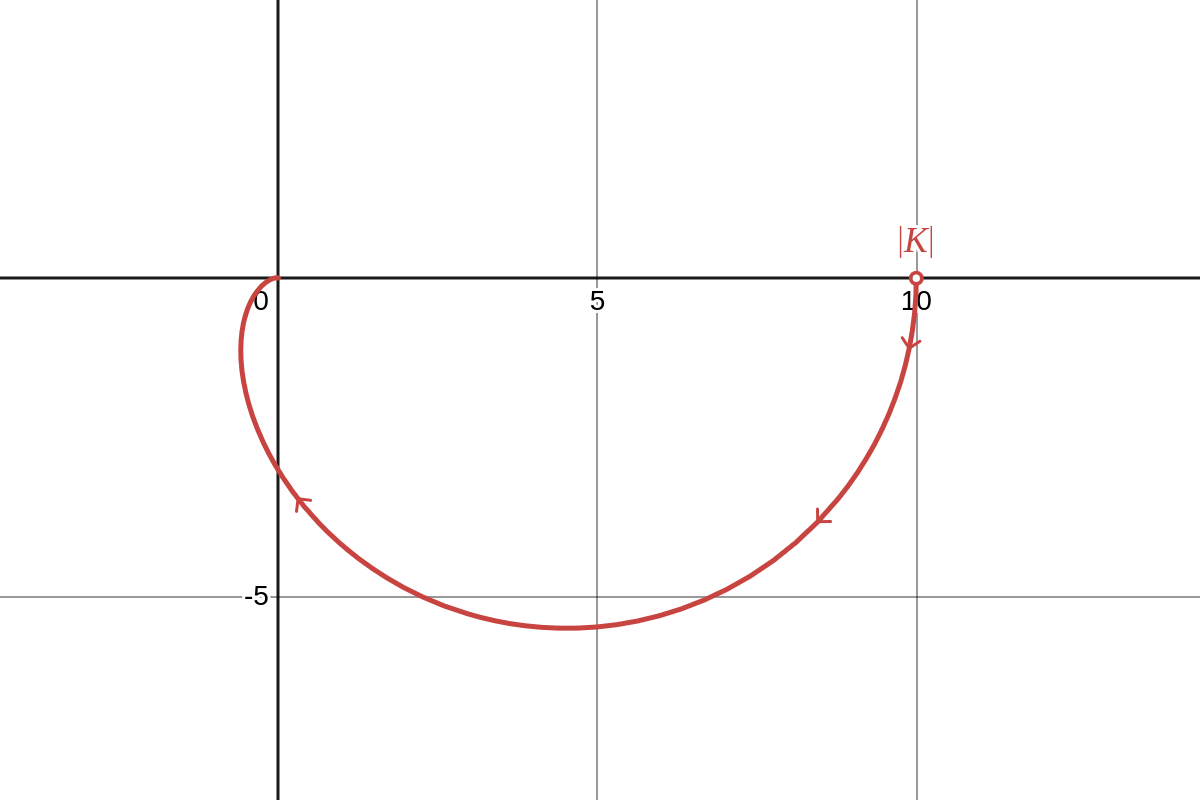
\includegraphics[scale=0.28]{../figures/nyquist/second_ex_3.png}
\end{center}

\end{document}
